% The step mapping chi on one row [FIPS 202, §3.2.4, Figure 6]:
% a'[x] = a[x] XOR ((NOT a[x+1]) AND a[x+2]).
% Original drawing for the Hash library.
\documentclass[tikz,border=6pt]{standalone}
\usepackage[T1]{fontenc}
\usepackage{lmodern}
% Shared style for the Hash diagrams.
% Palette: Okabe–Ito (colour-blind safe). Every diagram is drawn on an opaque white card so it
% stays legible on dark page themes.
\usetikzlibrary{arrows.meta,positioning,calc,fit,backgrounds}
\definecolor{hsblue}{HTML}{0072B2}
\definecolor{hsorange}{HTML}{E69F00}
\definecolor{hsgreen}{HTML}{009E73}
\definecolor{hsvermilion}{HTML}{D55E00}
\definecolor{hspurple}{HTML}{CC79A7}
\definecolor{hsink}{HTML}{1F2933}
\tikzset{
  >={Stealth[length=2.2mm]},
  every node/.style={font=\sffamily\small, text=hsink},
  wire/.style={draw=hsink, line width=0.6pt, ->},
  reg/.style={draw=hsink, line width=0.6pt, fill=hsblue!12, minimum width=9mm, minimum height=7mm},
  fn/.style={draw=hsink, line width=0.6pt, fill=hsorange!25, rounded corners=2pt, minimum width=10mm, minimum height=6mm},
  input/.style={draw=hsink, line width=0.6pt, fill=hsgreen!20, minimum width=9mm, minimum height=6mm},
  add/.style={circle, draw=hsink, line width=0.6pt, fill=white, inner sep=0pt, minimum size=5mm, font=\sffamily\bfseries},
  card/.style={fill=white, rounded corners=4pt},
}

\begin{document}
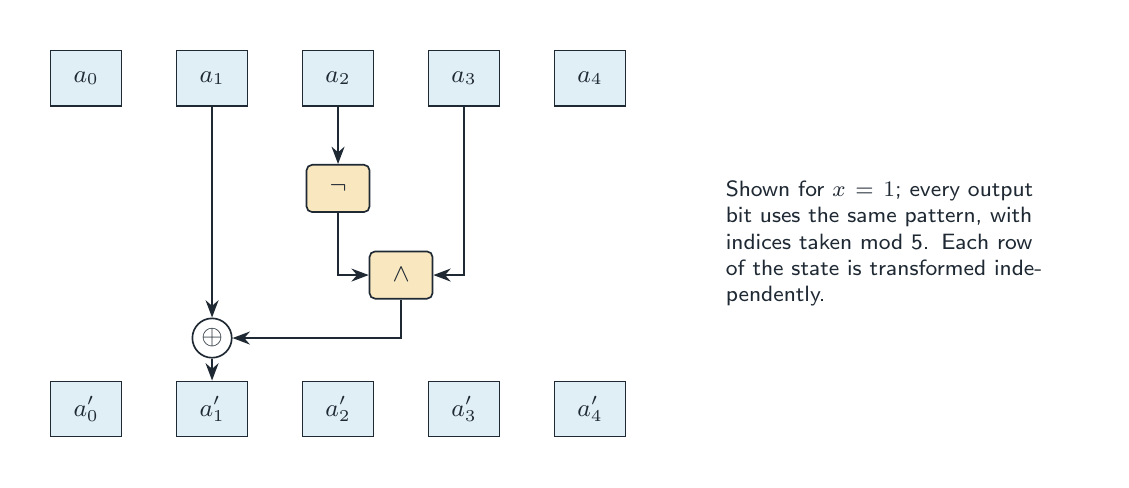
\begin{tikzpicture}
  \def\dx{1.6}
  \foreach \i in {0,...,4} {
    \node[reg] (a\i) at (\i*\dx, 0) {$a_{\i}$};
    \node[reg] (o\i) at (\i*\dx, -4.2) {$a'_{\i}$};
  }
  % Gates for output x = 1, using a1, a2, a3.
  \node[fn, minimum width=8mm] (n) at (2*\dx, -1.4) {$\neg$};
  \node[fn, minimum width=8mm] (and) at (2.5*\dx, -2.5) {$\wedge$};
  \node[add] (x) at (1*\dx, -3.3) {$\oplus$};
  \draw[wire] (a2.south) -- (n.north);
  \draw[wire] (n.south) |- (and.west);
  \draw[wire] (a3.south) |- (and.east);
  \draw[wire] (and.south) |- (x.east);
  \draw[wire] (a1.south) -- (x.north);
  \draw[wire] (x.south) -- (o1.north);
  \node[anchor=west, font=\sffamily\footnotesize, text width=4.2cm] at (5.0*\dx, -2.1)
    {Shown for $x = 1$; every output bit uses the same pattern, with indices taken mod 5. Each row of the state is transformed independently.};
  \begin{scope}[on background layer]
    \coordinate (e1) at (5.0*\dx+4.6, -1.0);
    \node[card, fit=(a0)(o4)(e1), inner sep=8pt] {};
  \end{scope}
\end{tikzpicture}
\end{document}
